\chapter{生成对抗网络与图像翻译}

\section{生成对抗网络基本原理}

生成对抗网络(GAN\cite{goodfellow2014generative})主要由生成器$G$和判别器$D$组成,将随机噪声$z$输入到生成器$G$中,输出相应的合成样本$G(z)$,生成器生成的分布假设为$G(z;\theta)$,$G(z)$可看作是对此分布的采样,同时事先知道真实样本集的分布$P_{data}$,在其中采样得到真实样本$x$。训练的时候,如图\ref{GAN}所示,随机噪声$z$经过生成器$G$得生成样本$G(z)$,判别器的输入为生成样本$G(z)$或真实样本$x$,输出为$D(G(z))$或$D(x)$,判别输入样本来自生成样本还是真实样本。在训练中,生成器的优化目标是尽可能生成可以骗过判别器的样本,判别器的优化目标则是尽可能将生成样本判为假,将真实样本判为真,生成器和判别器在优化目标上的矛盾决定了它们之间的对抗关系,可看成最大最小博弈,GAN的目标函数如下:
\begin{equation}
\begin{split}
\min \limits_{G} \max \limits_{D} V(D,G) = \mathbb{E}_{x\sim p_{data}(x)}[\log D(x)] + \mathbb{E}_{z\sim p_z(z)}[\log(1 - D(G(z)))]
\end{split}
\label{eq:GAN}
\end{equation}
其中$P_{data}$代表真实样本分布,$P_z$代表噪声分布。
% ,第一项表示判别器对真实样本的判断,第二项表示判别器对生成样本的判断。

\begin{figure}[ht]
    \centering
	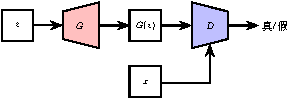
\includegraphics[width=.8\textwidth]{figs/GAN.pdf}
	\caption{GAN模型示意图\cite{goodfellow2014generative}。}
	\label{GAN}
\end{figure}

生成对抗网络相比较其它生成模型,优点在于:只用到了反向传播和梯度下降;可生成更逼真的样本;在应用方面,因其是非配对的训练方式,所以可以很自然地应用到无监督和半监督学习中;在设计损失函数方面,对于图像超分辨率、图像修复、图像去噪和风格迁移等任务上,无需根据任务的不同去精心设计损失函数,只需要给定想要达到的基准图像即可,判别器自会尽力生成高质量图像,避免了损失函数的设计困难。但生成对抗网络也有其缺点:因在训练时需要交替训练生成器和判别器,所以容易造成训练不稳定,难以达到纳什平衡;在训练时,判别器训练得比生成器快,当判别器训练得很好时,能很容易区别出真实样本和生成样本,从而出现梯度消失的问题;当生成器生成的样本仅代表真实样本的部分模式就可以欺骗判别器时,会导致生成样本缺乏多样性,出现模式崩塌。针对GAN存在的一系列问题,研究者们在GAN的基础上提出了各种变体或训练技巧加以避免。

\section{生成对抗网络变体}

GAN自提出后大受追捧,虽然可以生成比其它生成模型更清晰的图像,但仍存在一些问题,如:(1)生成器和判别器训练程度不对等,判别器训练得快且好,导致训练初期生成器的梯度容易消失,进而使生成器的参数基本不会更新;(2)训练不稳定,容易出现模式崩塌,生成器产生无意义的输出。研究者考虑GAN存在的问题以及可挖掘的空间,提出一系列GAN的变体模型。

\subsection{条件生成对抗网络}

原始GAN的输入是随机噪声,且无需预先建模,因此无法控制生成器的输出,2014年Mirza等人\cite{mirza2014conditional}提出的条件生成对抗网络(CGAN)在GAN的基础上给$G$和$D$加入额外的条件变量$y$,$y$在此起到约束和指引的作用,使生成样本可控。

\begin{figure}[ht]
    \centering
	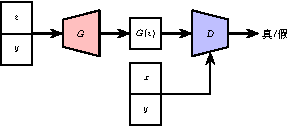
\includegraphics[width=.8\textwidth]{figs/CGAN.pdf}
	\caption{CGAN模型示意图\cite{mirza2014conditional}。}
	\label{CGAN}
\end{figure}

当加入条件变量$y$后,CGAN的目标函数为:
\begin{equation}
\begin{split}
\min \limits_{G} \max \limits_{D} V(D,G) = \mathbb{E}_{x\sim p_{data}(x)}[\log D(x|y)] + \mathbb{E}_{z\sim p_z(z)}[\log(1 - D(G(z|y)))]
\end{split}
\label{eq:CGAN}
\end{equation}

具体来说(如图\ref{CGAN}所示),假如$y$为类别标签,先将$y$进行one-hot编码,然后与随机噪声$z$按通道拼接,拼接后的编码输入生成器,得生成图像$G(z|y)$,判别器也用相似的处理方式将真实样本$x$或生成样本$G(z|y)$与$y$融合,判别器的输出$D(x|y)$或$D(G(z|y))$表明输入图像为真或假的概率。



\subsection{深度卷积生成对抗网络}

GAN中G和D的网络结构由简单的全连接层构成,存在难以训练的问题,深度卷积生成对抗网络(DCGAN)主要从网络结构上对GAN做改进。卷积神经网络(CNN)的开山之作是LeNet-5\cite{lecun1998gradient},在2012年ImageNet比赛上凭借AlexNet\cite{krizhevsky2012imagenet}大放异彩,从此广泛应用于计算机视觉领域。2016年Radford等人\cite{radford2015unsupervised}提出深度卷积生成对抗网络,将CNN引入$G$和$D$的网络结构中(如图\ref{DCGAN}),因为CNN之前多用于监督学习任务,而GAN是无监督学习,直接用卷积层替换全连接层并不能保证训练正常进行,经过探索,DCGAN确定了一个可以保证训练正常进行的方案:

(1)$G$和$D$中没有池化层和上采样层,转而用带步长的卷积代替,具体分为$D$用步长卷积,$G$中用反卷积,以提高训练的稳定性;

(2)在$G$和$D$中几乎每一层都用到批归一化(BN\cite{ioffe2015batch}),防止$G$把所有样本收敛到一个点,但直接将BN应用到所有层会导致模型不稳定,因此$G$的最后一层和$D$的第一层不加BN;

(3)移除全连接隐藏层,以构建更深层网络;

(4)$G$中使用$ReLU$\cite{nair2010rectified}激活函数,除了最后一层采用的是$Tanh$激活函数;

(5)$D$中所有层采用$LeakyReLU$\cite{xu2015empirical}激活函数。

DCGAN提出的网络结构不仅能够稳定训练,还能生成高质量图像,同时学习有意义的分解表示,可用于监督学习和生成建模。

\begin{figure}[ht]
    \centering
	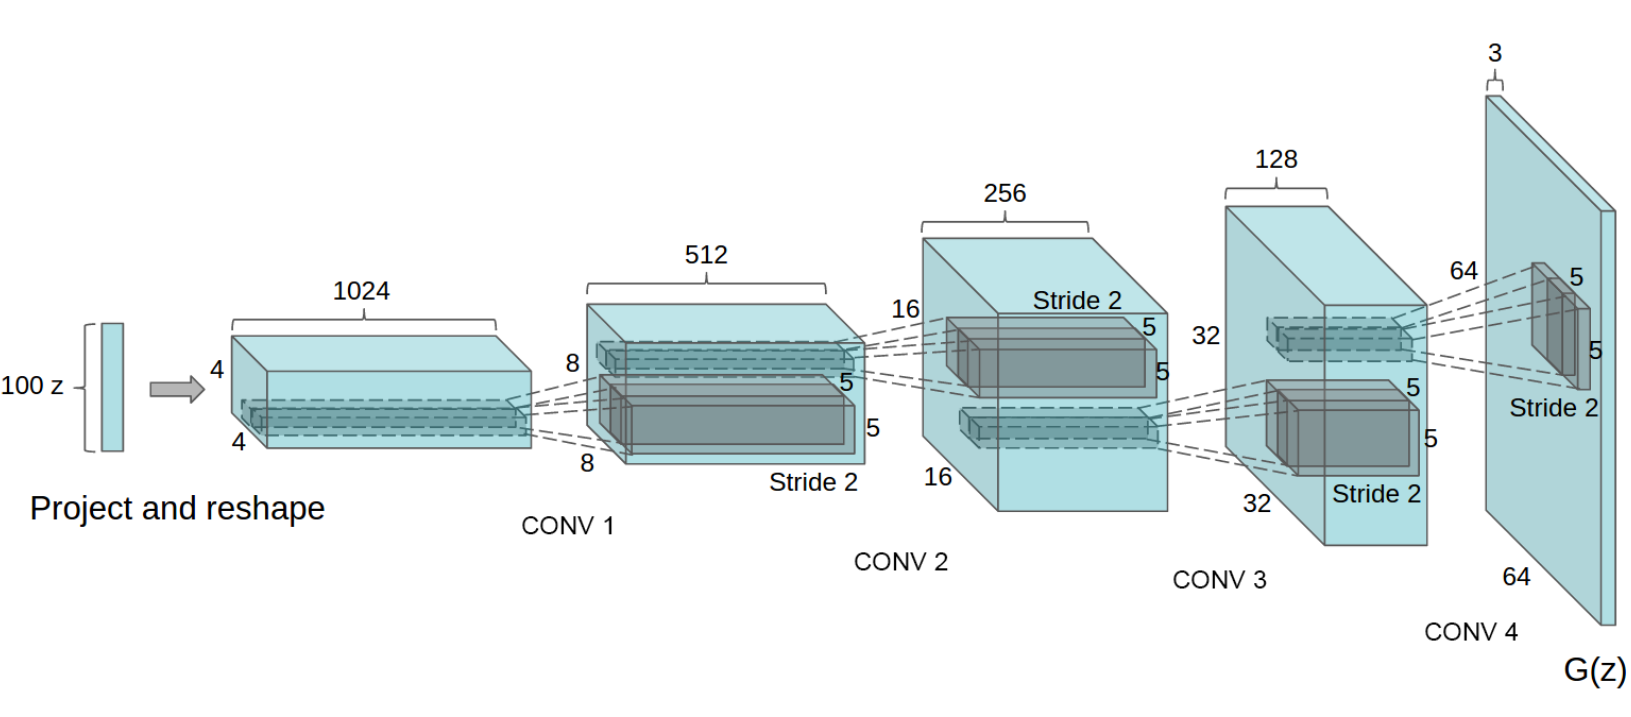
\includegraphics[width=\textwidth]{figs/DCGAN.png}
	\caption{DCGAN生成器结构示意图。图片来自文献\cite{radford2015unsupervised}。}
	\label{DCGAN}
\end{figure}

\subsection{结合变分自编码器的生成对抗网络}

VAE-GAN\cite{larsen2016autoencoding}提出了一种结合变分自编码器的生成对抗网络,如果只用VAE\cite{kingma2013auto}生成图像,容易产生模糊的结果,但生成结果有较高的多样性,如果只用GAN\cite{goodfellow2014generative},虽然能提高生成质量,但容易模式崩塌。VAE-GAN充分发挥这两种生成模型的优势,如图\ref{VAE-GAN}所示,VAE中的编码器将输入图像编码为均值和方差,利用均值和方差得到一个分布,并从此分布中采样得隐向量$z$,$z$经解码器生成$G(z)$。VAE的损失函数由两部分组成:确保生成图像和输入图像有一定相似性的损失和保证隐向量服从高斯分布的损失。VAE-GAN将VAE用作GAN的生成器,再加入一个判别器,用于判别输入图像的真假,VAE-GAN损失函数为VAE和GAN的损失函数之和。实验证明,VAE-GAN的生成效果比单独使用VAE或GAN好。

\begin{figure}[ht]
    \centering
	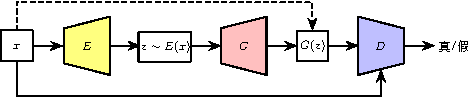
\includegraphics[width=\textwidth]{figs/VAEGAN.pdf}
	\caption{VAE-GAN模型示意图\cite{larsen2016autoencoding}。}
	\label{VAE-GAN}
\end{figure}

\section{基于生成对抗网络的图像翻译}

\subsection{配对图像翻译}
2017年Isola等人\cite{isola2017image}提出了基于条件生成对抗网络的图像翻译模型pix2pix,如图\ref{pix2pix}所示,整个网络架构中只有一个生成器$G$和一个判别器$D$,源域图像$x$经生成器$G$得生成的目标域图像$G(x)$,在判别时,源域图像作为条件辅助判别,其对抗损失函数类似于CGAN。

在pix2pix中,判别器的目的没有变化,但生成器的目的不仅是骗过判别器,还需要和真实图像尽可能相似,L1损失\cite{isola2017image}\cite{shrivastava2017learning}(公式\ref{eq:pix2pix_l1})相比较L2损失\cite{pathak2016context}可以在保证与真实图像相近的同时产生更少的模糊。
\begin{equation}
\begin{split}
\mathcal{L}_{L1}(G) = \mathbb{E}_{x,y,z}[\parallel y-G(x,z)\parallel_1]
\end{split}
\label{eq:pix2pix_l1}
\end{equation}

\begin{figure}[ht]
    \centering
	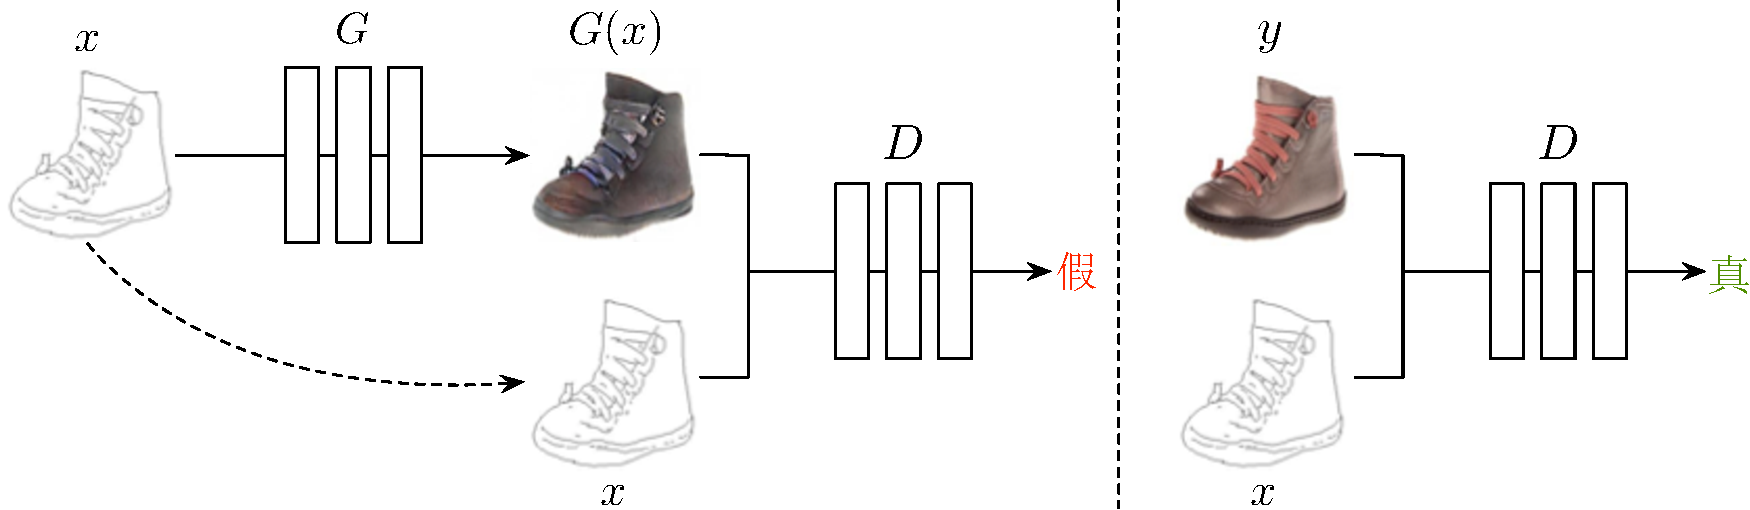
\includegraphics[width=\textwidth]{figs/pix2pix.pdf}
	\caption{Pix2pix训练示意图。图片来自文献\cite{isola2017image}。}
	\label{pix2pix}
\end{figure}

Isola等人认为虽然输入图像和输出图像外观上不同,但潜在结构应相似,输入和输出之间共享大量低级信息,因此生成器采用有跳连接的U-Net\cite{ronneberger2015u}结构,下采样过程中产生的特征图与上采样过程产生的同尺寸的特征图按通道拼接到一起,以此保留不同分辨率的信息,提高生成质量。Pix2pix的目标函数包含学习低频信息的重建损失和学习高频信息的对抗损失,既然对抗损失只解决高频信息,所以判别器采用的是PatchGAN结构,它不需要将整幅图像输入到判别器中,而是对每个大小为N$\times$N的区域做真假判别。

\begin{figure}[ht]
    \centering
	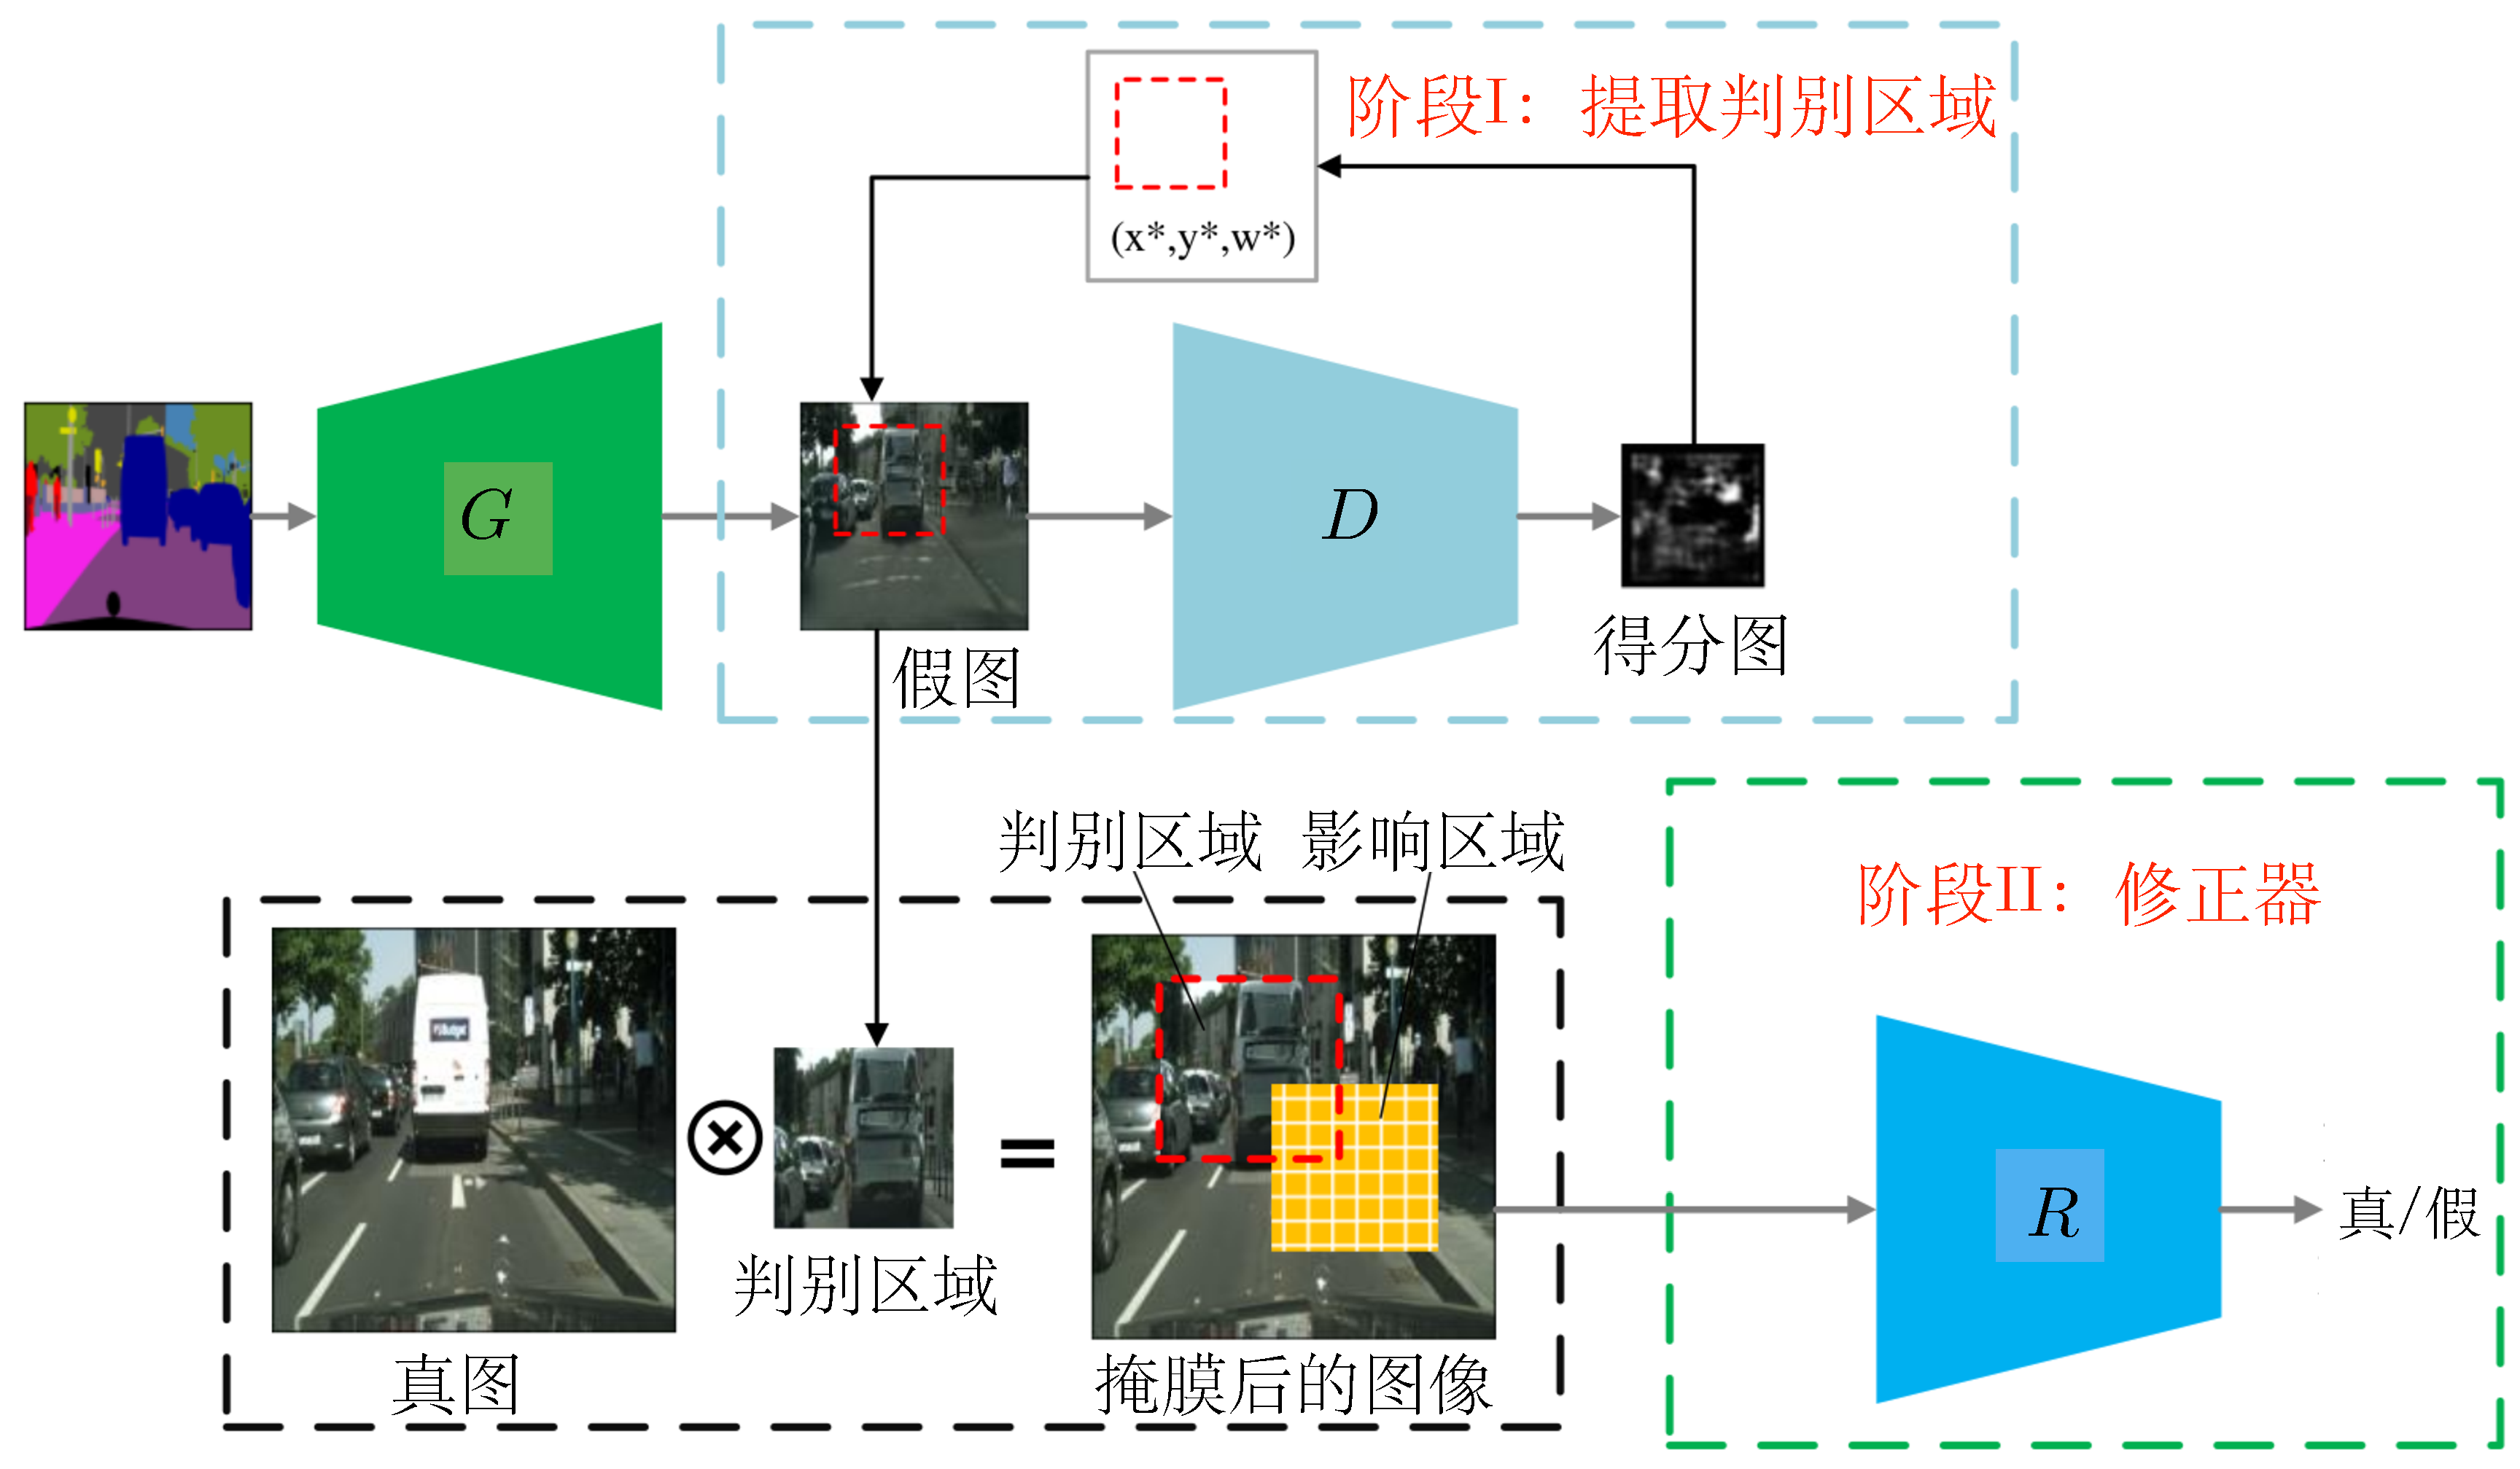
\includegraphics[width=.9\textwidth]{figs/DRPAN.pdf}
	\caption{DRPAN训练示意图。图片来自文献\cite{wang2019discriminative}。}
	\label{DRPAN}
\end{figure}

Wang等人\cite{wang2019discriminative}考虑图像翻译任务中仍存在的失真、形变和拉伸等问题,提出DRPAN以得到高质量和高分辨率的图像翻译结果。如图\ref{DRPAN}所示,整个网络由三部分组成:生成器$G$、判别器$D$和修正器$R$。输入图像经生成器得到假图,随后假图进入判别器,此判别器在PatchGAN的基础上扩展为一个判别区域建议网络,主要用于输出反映生成图像真实程度的得分图,然后通过滑动窗口找到并提取假图中得分较低的区域,即图\ref{DRPAN}中的判别区域。判别区域与真图做掩膜操作得到掩膜后的假图,然后将真图和掩膜后的假图输入修正器中做优化训练,修正器可以对一幅图像不同的区域进行迭代式更新优化。将掩膜后的图像输入修正器的行为可看作一种直接的注意力机制,让修正器专注于修正合成效果不好的位置。

SPADE\cite{park2019semantic}提出一个简单但有效的层:空间自适应归一化,可用于将语义分割图翻译成图像。之前的工作是将语义分割图作为输入直接喂入网络中,然后通过卷积层、归一化层和非线性激活函数处理,但这易于“冲走”语义信息。为了解决此问题,SPADE提出了空间自适应归一化,用学习到的缩放和偏差进行调制。输入图像经编码器得到与其分布有关的均值和方差,然后利用此均值和方差与高斯分布进行反归一化,得到一个包含真实图像信息的随机向量,生成器以随机向量为输入,并在此过程中不断加入语义分割图以利用SPADE增强语义信息,最终得到逼真的图像。

虽然上述方法可以生成高质量图像,但它需要配对数据集,而配对数据集的获取十分困难,而且对于一些任务,获取配对数据集是不可能的,如照片转莫奈画,马转斑马等,因此需要一种可以实现非配对图像翻译的方法。

\subsection{非配对图像翻译与循环一致}

Zhu等人\cite{zhu2017unpaired}提出的CycleGAN能够在没有配对数据的情况下,在源域和目标域之间建立一个确定的映射,实现图像翻译。给定源域$X$和目标域$Y$,利用生成器$G$学习从$X$到$Y$的映射$G:X\to Y$,即给定来自$X$域的图像$x$,经此映射可得$Y$域的生成图像$\hat{y}=G(x)$,理论上,$\hat{y}$应与真实样本的分布$p_{data}(y)$相匹配,最优$G$将图像从$X$域翻译到与$Y$域相近的$\hat{Y}$域,但实际上,由于缺乏配对数据集提供的约束,$G:X\to Y$映射并不能保证输入$x$与输出$y$以有意义的方式配对,即无法保证$G$是单一的,这容易导致模式崩塌。针对这一问题,zhu等人提出再增加一个映射$F:Y\to X$,$G$和$F$的网络结构一致,除此之外,还引入循环一致性损失用于确保$F(G(x)) \approx x$和$G(F(y)) \approx y$,损失函数定义为:
\begin{equation}
\begin{split} 
\mathcal{L}_{cyc}(G, F) = \mathbb{E}_{x\sim p_{data}(x)}[\parallel F(G(x)) - x\parallel_1] + \mathbb{E}_{y\sim p_{data}(y)}[\parallel G(F(y)) - y\parallel_1]
\end{split}
\label{eq:pix2pix}
\end{equation}
与两个生成器相对应,CycleGAN还引入有相同结构的判别器$D_X$和$D_Y$,用于对$X$域和$Y$域的判别,总损失函数是循环一致性损失和对抗损失的和。

\begin{figure}[ht]
    \centering
	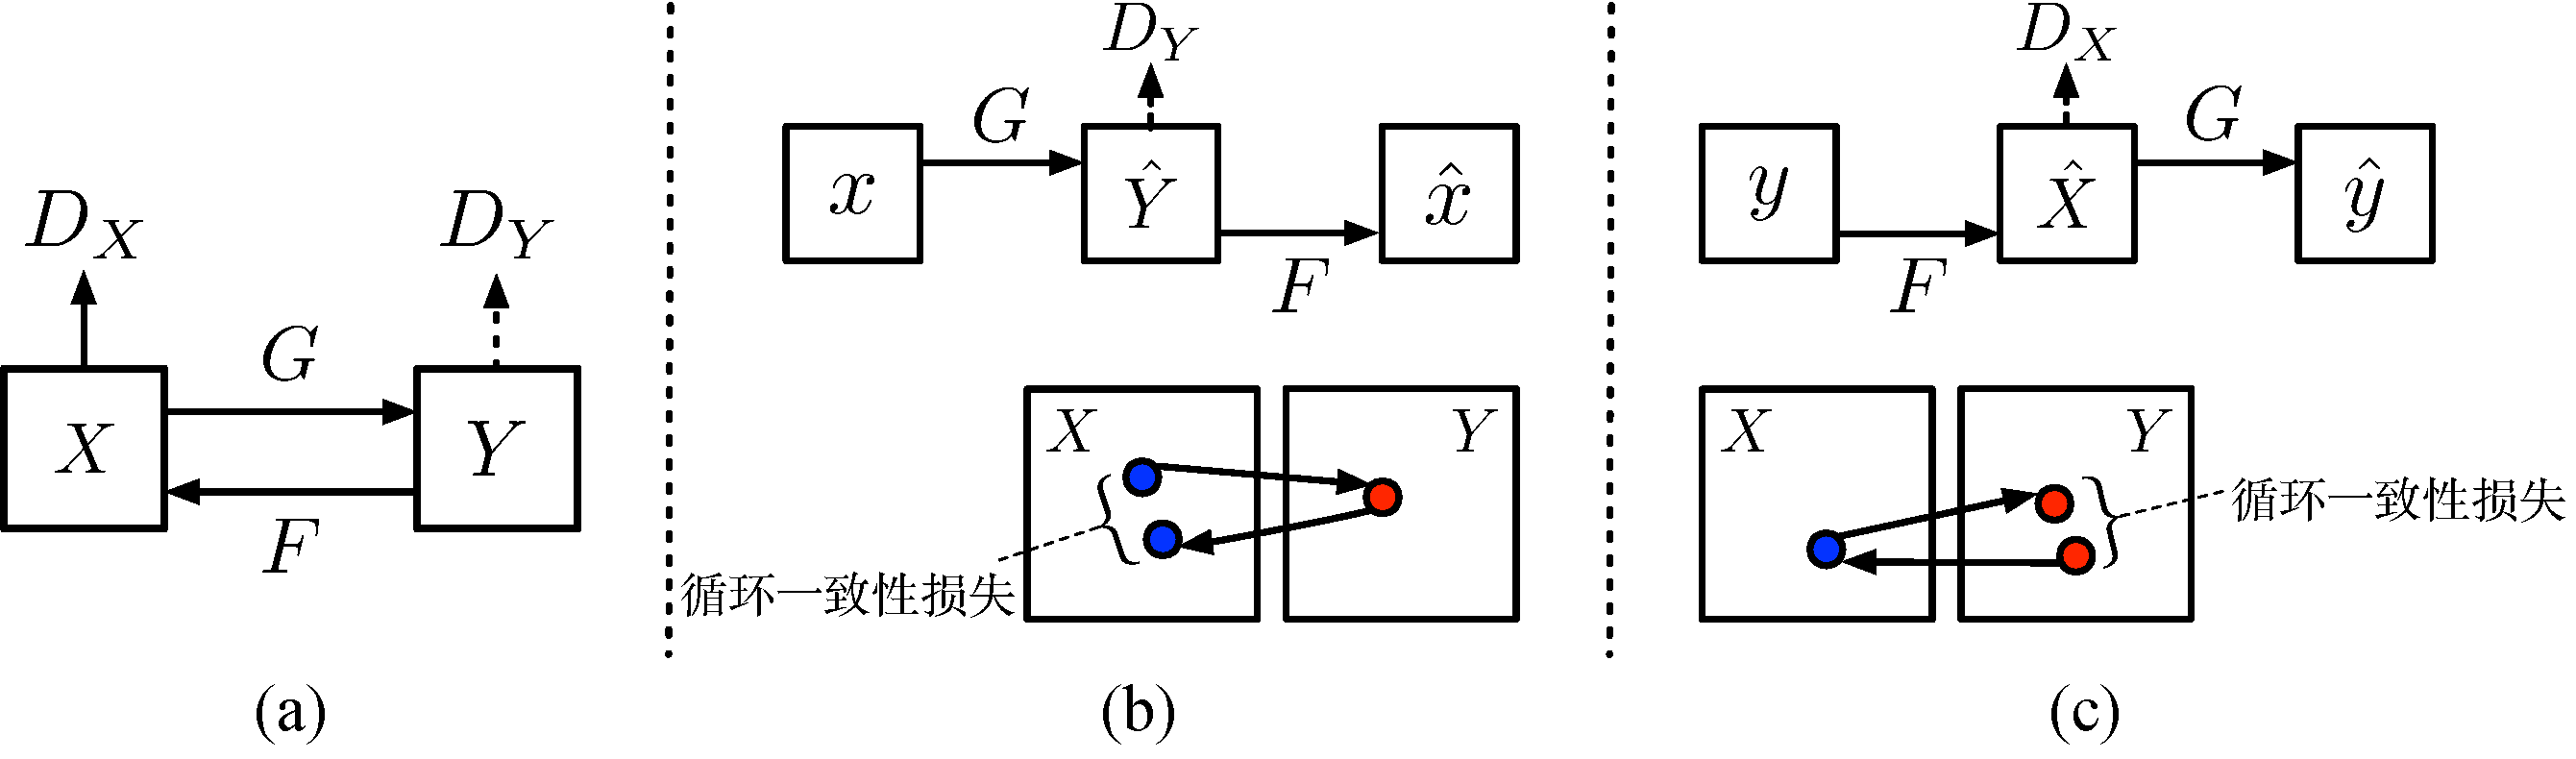
\includegraphics[width=\textwidth]{figs/cyclegan.pdf}
	\caption{CycleGAN训练示意图。图片来自文献\cite{zhu2017unpaired}。}
	\label{CycleGAN}
\end{figure}

CycleGAN在马和斑马、季节变化、照片和画作等任务上均性能优异,验证了CycleGAN的广泛适用性和有效性。使用循环一致性损失的还有Kim等人\cite{kim2017learning}提出的DiscoGAN和Yi等人\cite{yi2017dualgan}提出的DualGAN,它们的方法和思想类似,此处不再展开介绍。

Liu等人提出的UNIT\cite{liu2017unsupervised}将非配对图像翻译定义为知道边缘概率密度,学习联合概率密度的问题,但这是一个高度不适定问题,对此,UNIT提出一种共享潜在空间的假设。假定$X_1$和$X_2$分别表示两个图像域,图像$x_1\in X_1$和$x_2\in X_2$可分别经过编码器$E_1$和$E_2$被映射到相同的潜码$z$,生成器$G_1$和$G_2$可再将潜码$z$解码回相应的$x_1$和$x_2$。为了实现共享潜在空间,UNIT利用权重共享策略,将编码器的后几层连接到一起,生成器的前几层也连接到一起。UNIT在白天转黑夜、动物脸翻译等任务上表现较好,但它的输出只能是单模态的,不能实现一对多翻译。

\subsection{非配对图像翻译与分解表示}

Huang等人提出的MUNIT\cite{huang2018multimodal}将一幅图像分解到代表底层空间结构的内容隐空间和代表结构渲染的风格隐空间,文中假设两个域共享同一个内容隐空间,风格隐空间是特定于域的,如\ref{MUNIT}所示,$x_1 \in X_1$和$x_2 \in X_2$是来自两个域的图像,$c_i$和$s_i$分别是由$x_i$经两个编码器得到的内容隐编码和风格隐编码。为了实现从$X_1$到$X_2$域的翻译,MUNIT将提取的内容隐编码$c_1=E_1^c(x_1)$和从先验分布$q(s_2)\sim\mathcal{N}(0, \mathbf{I})$中随机采样的风格隐编码输入到生成器$G_2$中,以产生最终的输出图像$x_{1\to2}=G_2(c_1,s_2)$。

\begin{figure}[ht]
    \centering
	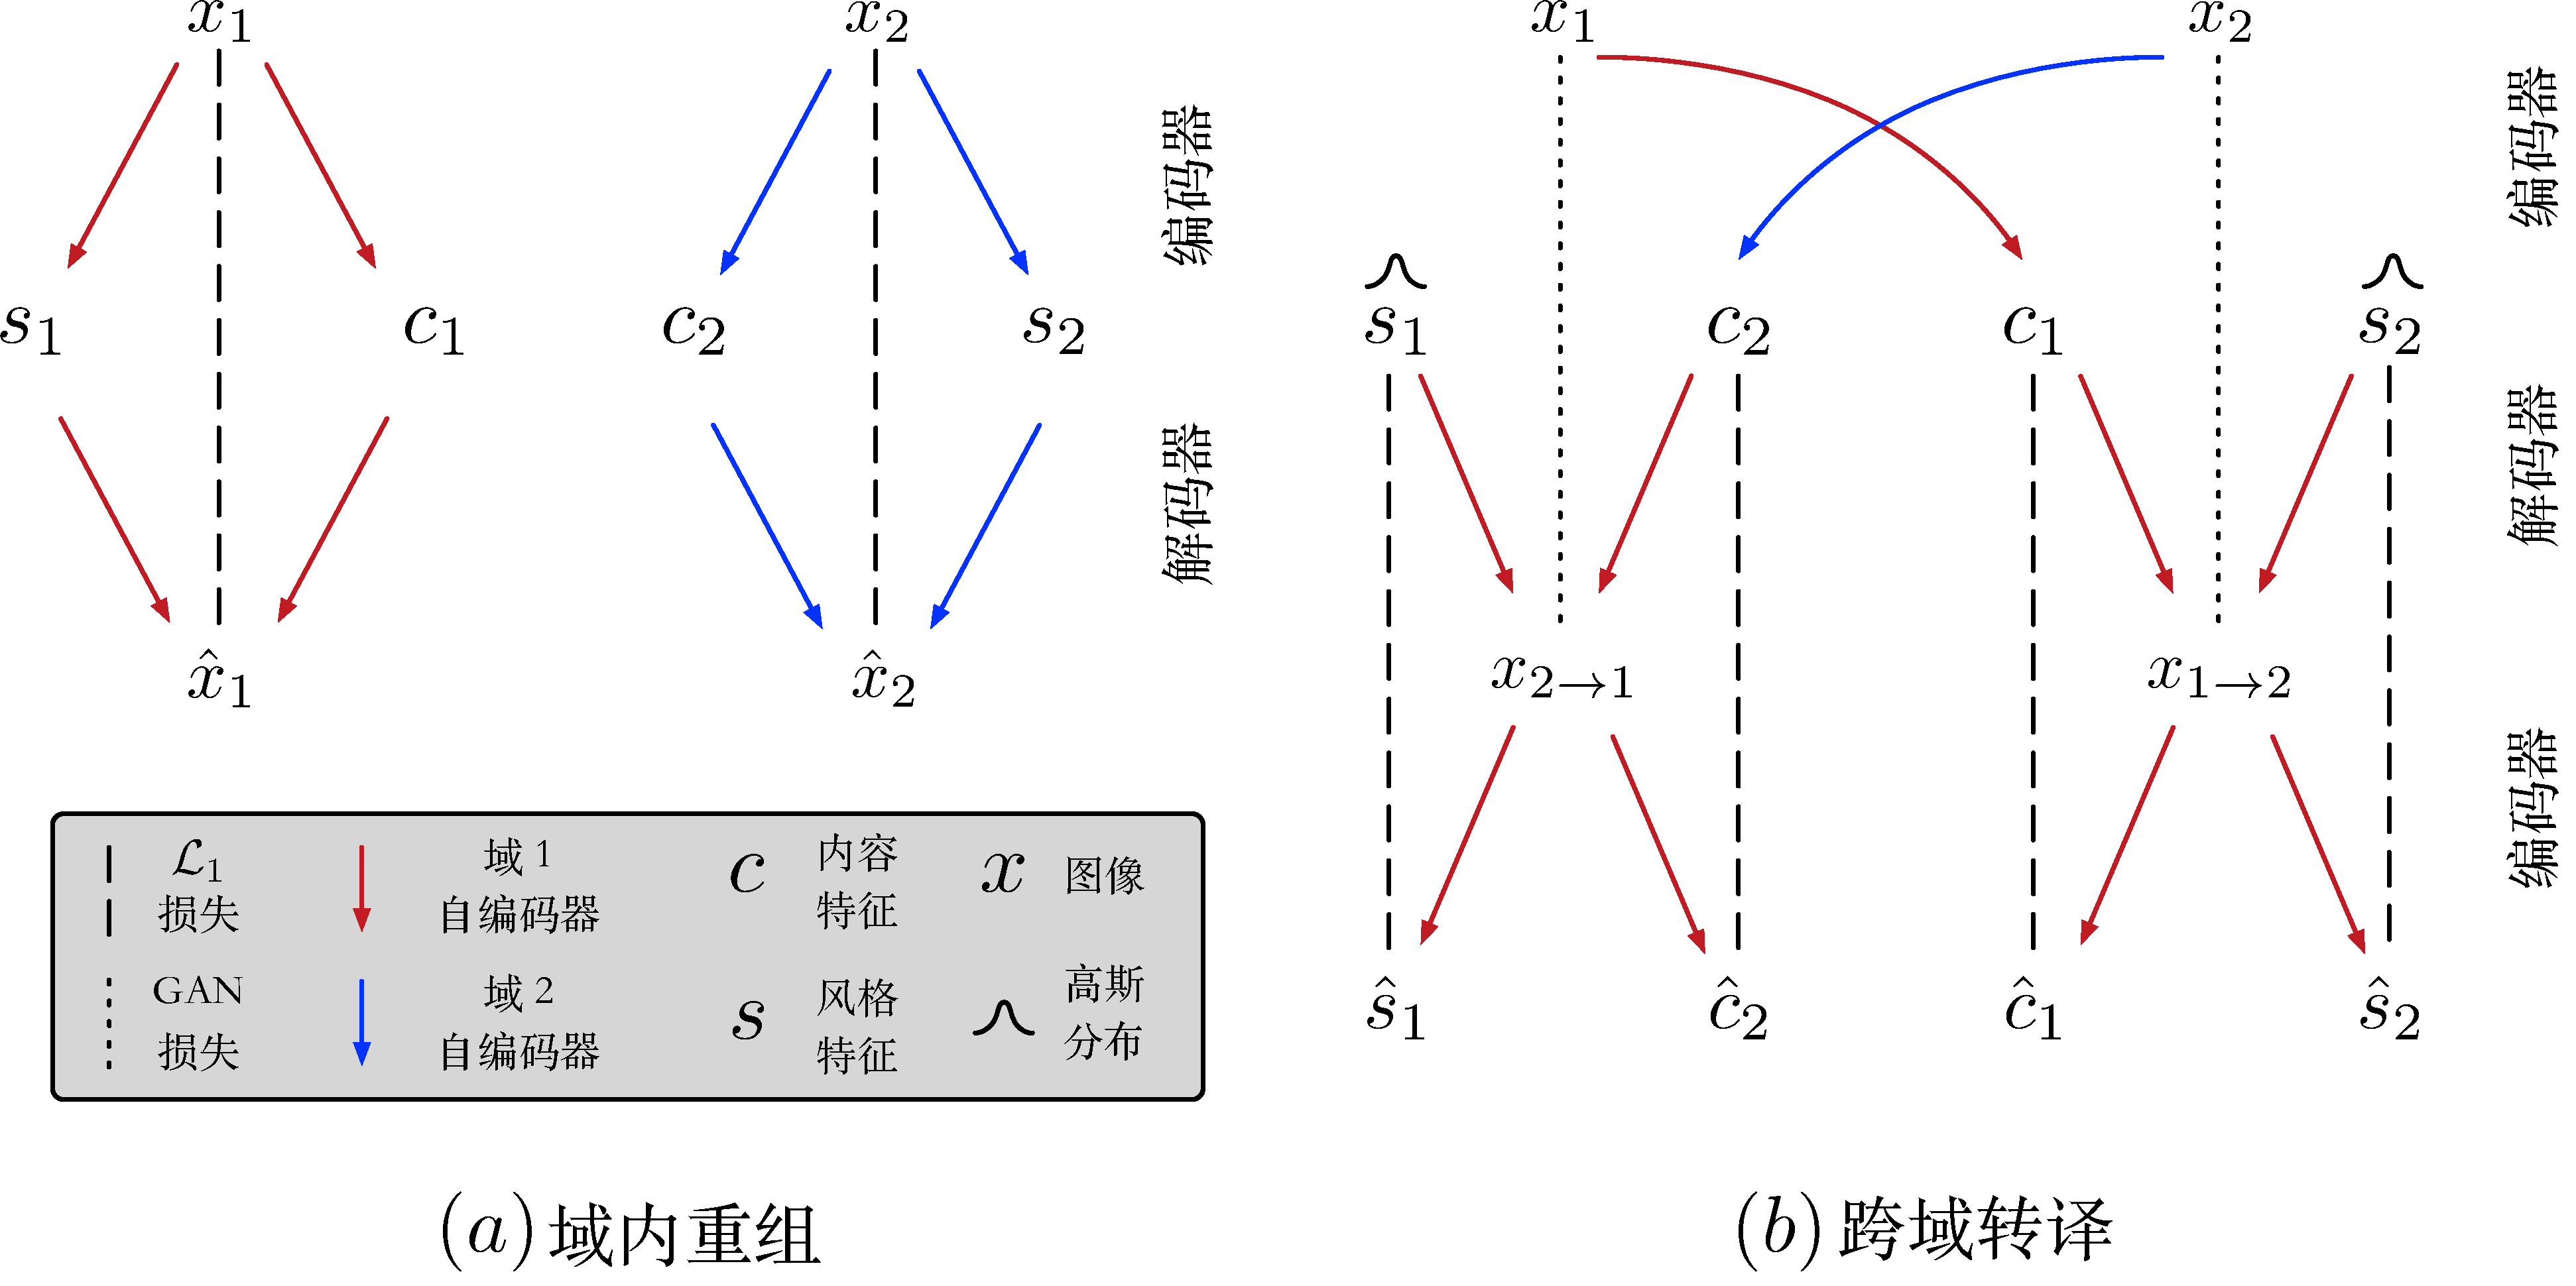
\includegraphics[width=\textwidth]{figs/MUNIT.pdf}
	\caption{MUNIT训练示意图。图片来自文献\cite{huang2018multimodal}。}
	\label{MUNIT}
\end{figure}

MUNIT的损失函数包括对抗损失和双向重建损失,对抗损失使生成图像的分布尽量逼近目标域的图像分布,双向重建损失则用于确保配对的编码器和解码器互逆。双向重建损失包含对图像的重建和对潜码的重建:给定一个源域图像,经过编码和解码后可重建出此源域图像;给定一个从潜在空间采样的潜码,经过解码和再次编码,应该重建出此潜码。

Lee等人提出的DRIT\cite{lee2018diverse}与MUNIT类似,也假设有一个捕捉不同域之间共同信息的域不变内容隐空间和两个特定于域的属性隐空间,图\ref{DRIT}中的$\{E_X^c, E_Y^c\}$和$\{E_X^a, E_Y^a\}$分别为两个域的内容编码器和属性编码器,$G_X$和$G_Y$是生成器,用于将内容隐编码和属性隐编码整合并生成图像。

为了实现分解表示,将两个内容编码映射到同一隐空间中,DRIT采用权重共享和内容判别策略,共享$E_X^c$和$E_Y^c$的最后一层以及$G_{X}$和$G_{Y}$的第一层权重,通过权重共享,将内容表示强制映射到同一空间。但共享相同的高级映射函数并不能保证可将不同域的内容表示成相同的内容编码,因此还引入用于判别内容编码$z_x^c$和$z_y^c$的判别器$D^c$。

\begin{figure}[ht]
    \centering
	\includegraphics[width=\textwidth]{figs/DRIT.pdf}
	\caption{DRIT训练示意图。图片来自文献\cite{lee2018diverse}。}
	\label{DRIT}
\end{figure}

MUNIT和DRIT都采用分解表示的方式实现多模态输出,是多模态图像翻译方面的经典之作,后续产生一系列在它们基础上改进的工作。Mao等人提出的MSGAN\cite{mao2019mode}设计了一个简单但有效的模式搜寻正则化项,其主要思想是最大化输出图像之间的距离与输入的隐空间之间的距离的比值,可解决CGAN模式崩塌问题。这一正则化项很容易扩展到现有框架中,在非配对图像翻译中,MSGAN在DRIT上加入模式搜寻正则化项,可得到更多样和更高质量的图像。

给定一个来自隐编码空间$Z$的隐向量$z$,将其映射到图像空间$I$中,当网络发生模式崩塌时,输出图像只有少量模式,即当两个隐向量$z_1$和$z_2$很接近时,映射得到的两个图像$I_1=G(c,z_1)$和$I_2=G(c,z_2)$更趋向于有相同的模式。为解决此问题,MSGAN提出模式搜寻正则化项,旨在最大化$G(c,z_1)$和$G(c,z_2)$之间的距离与$z_1$和$z_2$之间的距离的比值:
\begin{equation}
\begin{split} 
\mathcal{L}_{ms}=\max\limits_{G}(\frac{d_I(G(c,z_1),G(c,z_2))}{d_z(z_1,z_2)}),
\end{split}
\label{eq:MSGAN}
\end{equation}
其中$d_{\ast}(\cdot)$表示距离度量。相比于DRIT从高斯分布中采样一个编码,为将模式搜寻正则化加入DRIT中,现从高斯分布中随机采样两个编码$z_1$和$z_2$,仅做一点改变就可输出更多样化的结果。

\begin{figure}[ht]
    \centering
	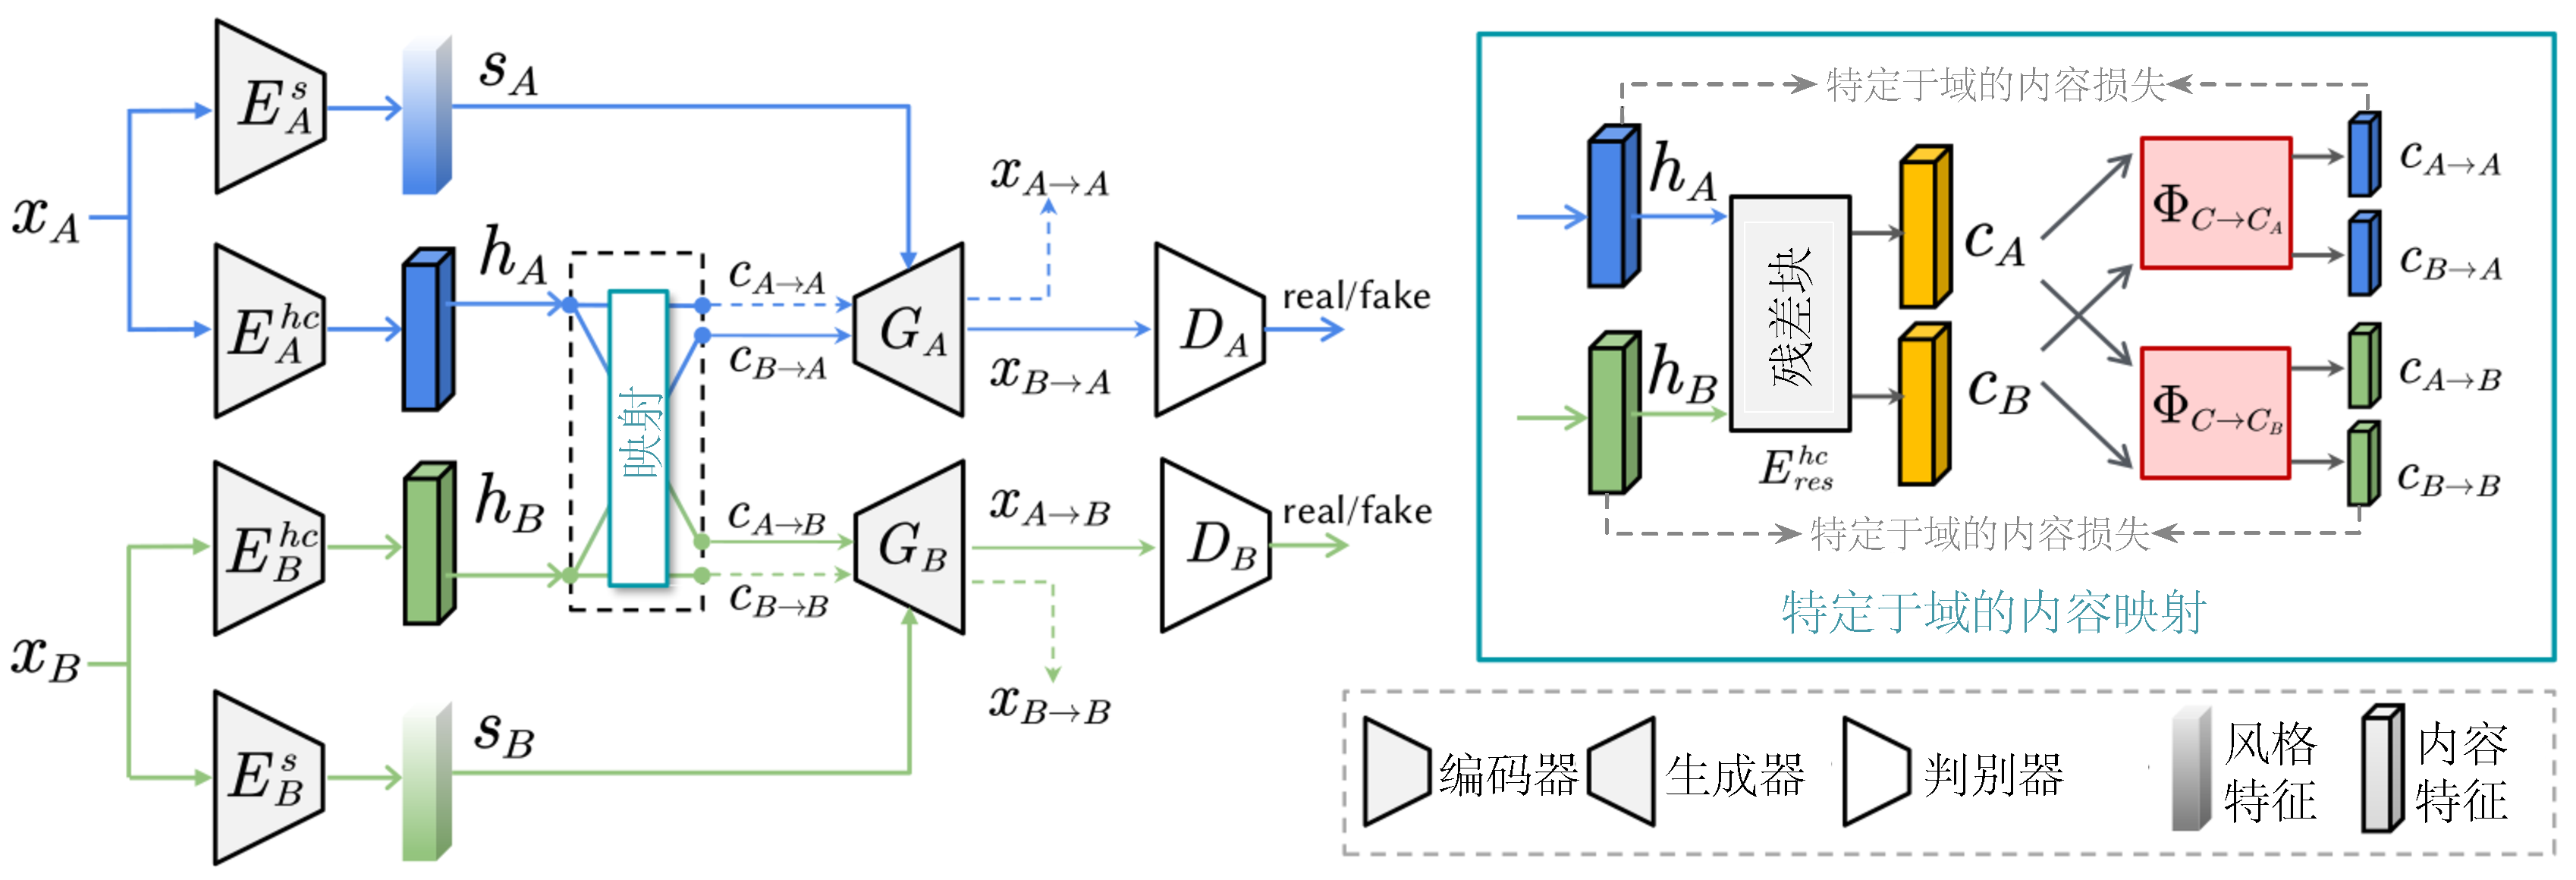
\includegraphics[width=\textwidth]{figs/DSMAP.pdf}
	\caption{DSMAP训练示意图。图片来自文献\cite{chang2020domain}。}
	\label{fig:DSMAP}
\end{figure}

Chang等人\cite{chang2020domain}提出的DSMAP在MUNIT的基础上,对共享的域不变内容空间中的潜在特征做进一步映射(如图\ref{fig:DSMAP}所示),将其重新映射到特定于域的内容空间中。DSMAP做此改进是因为作者观察到之前基于分解的方法不考虑内容和风格之间的关系,共享的域不变内容空间可能会限制表达内容的能力,因为域不变的内容特征可能包含域相关信息。

在两个域$X_A$和$X_B$中,除了基本的内容编码器$\{E_A^c, E_B^c\}$、风格编码器$\{E_A^s, E_B^s\}$和生成器$\{G_A, G_B\}$,DSMAP还引入两个额外的特定于域的映射函数$\Phi_{C\to C_A}$和$\Phi_{C\to C_B}$,它们将共享的域不变内容空间中的特征映射到特定于$X_A$域和$X_B$域的内容空间中。在$X_A\to X_B$的翻译中,内容来自于$X_A$,风格来自于$X_B$,内容编码器$E_A^c$将$x_A\in X_A$映射到为域不变内容特征$c_A=E_A^c(x_A)$,风格编码器$E_B^s$将$x_B\in X_B$映射到为特定于域的风格特征$s_B=E_B^s(x_B)$,MUNIT和DRIT通过生成器$G_B$得生成图像$x_{A\to B}=G_B(c_A, s_B)$。DSMAP认为这样简单地提取域不变内容特征$c_A$不足以生成高质量$X_B$域图像,最好在合成前就将$c_A$和目标域的内容特征对齐。因此,$\Phi_{C\to C_B}$将内容特征$c_A$映射到$X_B$的内容空间,然后生成器$G_B$利用内容特征$c_{A\to B}$和风格特征$s_B$合成最终的输出图像$x_{A\to B}$。总的来说,$X_A\to X_B$的生成过程为:
\begin{equation}
\begin{split} 
x_{A\to B}=\Phi_{X_A\to X_B}(x_A, x_B)=G_B(\Phi_{C\to C_B}(c_A), s_B),
\end{split}
\label{eq:DSMAP}
\end{equation}
DSMAP提出了一种分解特征再映射的想法,其可以提取更纯净的内容特征的特点使之在风格迁移任务上展示出更有说服力的结果。

\section{小结}

本章从生成对抗网络的原理展开,介绍了不同的生成对抗网络变体和多种基于生成对抗网络的图像翻译方法。

第一节主要介绍了生成对抗网络的原理和主要架构,指出GAN以博弈的方式提高了生成质量,但也伴随着模式崩塌、训练不稳定、生成图像的分辨率不高和生成样本多样性不足等问题。

第二节介绍了GAN的一系列变体,DCGAN和VAE-GAN等通过提出新的网络架构以保证GAN可以稳定训练,在一定程度上缓解了模式崩塌。

第三节介绍基于生成对抗网络的图像翻译方法,然后分析了配对图像翻译(包括pix2pix等)和非配对图像翻译(包括CycleGAN和DRIT等),重点介绍非配对图像翻译中的两种思想:循环一致和分解表示。

在逐步地深入介绍后,明确基于生成对抗网络的图像翻译的原理和应用,接下来将关注非配对图像翻译,利用循环一致和分解表示解决两个应用问题。